
%(BEGIN_QUESTION)
% Copyright 2011, Tony R. Kuphaldt, released under the Creative Commons Attribution License (v 1.0)
% This means you may do almost anything with this work of mine, so long as you give me proper credit

Skjermbildet under viser konfigurasjonsvindu for et HMI-panel med serielle kommunikasjonsparametere for datautveksling mot en Modbus-enhet:

$$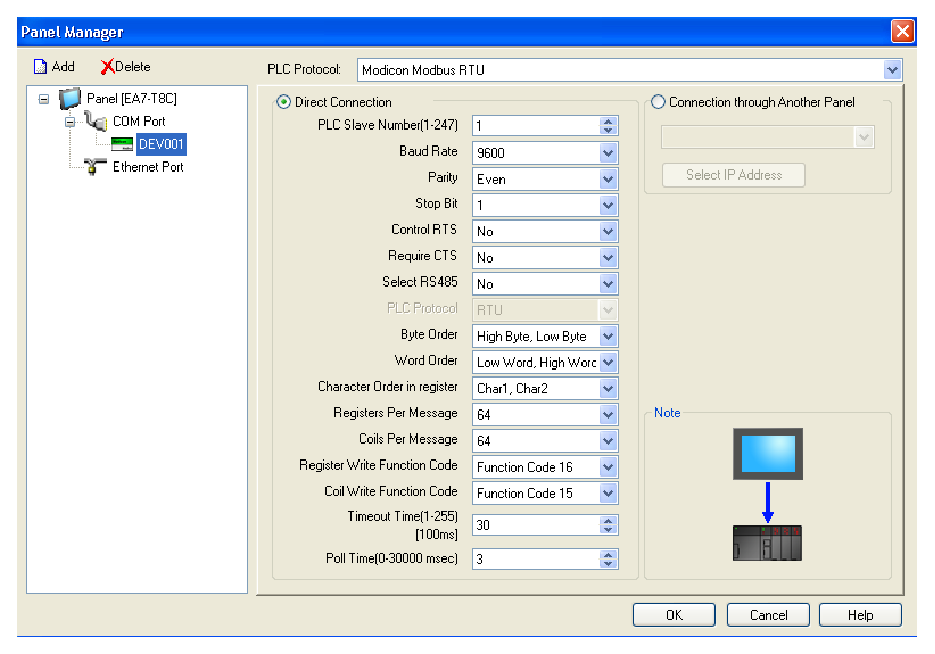
\includegraphics[width=15.5cm]{i00718x01.eps}$$

Identifiser hensikten med parameterne "Control RTS" og "Require CTS", som her er deaktivert ("Nei").

\vskip 50pt

Det finnes to valg for Modbus Register Write-funksjonskoder: 06 og 16. Tilsvarende finnes to valg for Modbus Coil Write: 05 og 15. Forklar forskjellen mellom valgene, og hvorfor én innstilling kan være mer nyttig enn en annen.

\vfil

\underbar{file i00718no}
\eject
%(END_QUESTION)





%(BEGIN_ANSWER)

Dette er en vurdert oppgave -- ingen svar eller hint er gitt!

%(END_ANSWER)





%(BEGIN_NOTES)

"Control RTS" og "Require CTS" er {\it handshaking}-signaler mellom HMI og serieenhet. "Request To Send" og "Clear To Send" sikrer at mottakeren er klar før sending starter. Handshaking bruker ekstra tid, derfor er det ofte avslått som standard.

\vskip 10pt

Modbus-kode 15 og 16 kan skrive {\it flere} coils/registere i én operasjon, mens 05 og 06 skriver {\it én} coil/register av gangen. Når mange punkter skal skrives effektivt, er 15/16 bedre enn 05/06.

%(END_NOTES)
